% Project Report Template. Antonio Carrasco-Munoz. Leeuwarden, 2022.
\documentclass[oneside,12pt]{article}
\usepackage[a4paper,width=150mm,top=25mm,bottom=25mm]{geometry}
\usepackage[utf8]{inputenc}
\usepackage[english]{babel}
\usepackage{graphicx}   \graphicspath{{figures/}}
\usepackage[margin=30pt,labelfont=bf,labelsep=period,font={small,stretch=1.1}]{caption} % Caption settings
\usepackage{setspace}
\usepackage[font={normal,stretch=1.1}]{subcaption}
\usepackage{amssymb,wasysym}% Symbols
% \usepackage[table,dvipsnames]{xcolor}     % Provides a common set of commands for color manipulation
\usepackage[hidelinks]{hyperref} % Links: table of contents, references, bibliography, figures, pages, url's, etc.
\usepackage{fancyhdr} \pagestyle{fancy} % Page heading
\fancyhead[L]{\nouppercase{\rightmark}} \fancyhead[R]{\nouppercase{\leftmark}} % No uppercase
\usepackage{array} % To control table cell width
\usepackage{makecell}
\usepackage[]{natbib} \bibliographystyle{apalike}    % Bibliography management
\usepackage{blindtext}
\usepackage{soul}
\usepackage{lscape}
\usepackage{color}
\usepackage{algpseudocode}
\usepackage{algorithm}
\newcommand{\un}[1]{\,\mathrm{#1}}
\algnewcommand{\LineComment}[1]{\State \(\triangleright\) #1}
\newcommand{\bigO}{\mathcal{O}}
\newcommand{\codeword}[1]{\texttt{\textcolor{blue}{#1}}}
\begin{document}

\setlength{\parindent}{0 em}    % Paragraph indentation
\setlength{\parskip}{0.7 em}    % Space between paragraph and preceding text
\renewcommand{\baselinestretch}{1.5}    % Line spacing

\newcommand{\ProjectTitle}{GETEC project} % <---Write here the project title!!!

\begin{titlepage}
    \begin{center}
    \vspace*{3 cm}
    \Huge
    \textbf{Report} \\
    \vspace{1 cm}    
    \textbf{\ProjectTitle} % Do not write here! Go higher, line 10.
    \\
    \vspace{1 cm}
    \vfill      % Automatically add in the amount of vertical space needed for the content to fill the page
    
\includegraphics[width=60mm]{figures/NHLStenden-logo.png} \\
    \end{center}
    \vspace{2 cm}
    \normalsize
    Title : \ProjectTitle % Do not write here! Go higher, line 10.
    \\
    Authors : Juliana G. R. de Carvalho, Luewton L F Agostinho, Alexander Finnegan, Janneke Dickhout
    \\
    Date : \today 
    \\
    Code : 
    \\
    Version : 1 \\
    Status : draft \\
    Mailing list : 
    \\
    Copy to : \\
    Classification : confidential
\end{titlepage}

% \chapter*{} \thispagestyle{empty}   % "Page break"
% \chapter*{} \thispagestyle{empty}   % "Page break"

% ---------- MAIN TEXT ---------- %
\setlength{\parindent}{0 em}  % Paragraph indentation
\setlength{\parskip}{0.7 em}    % Space between paragraph and preceding text

\newpage    \pagestyle{empty}
\tableofcontents
\pagestyle{fancy}


% ======== EXAMPLE OF FIGURE ============
% \begin{figure}[ht!]
%     \centering
%     \includegraphics[width=.9\textwidth,trim=1 1 1 1,clip]{Filamented_particles.png}
%     \caption{SEM images of polystyrene particles carrying filaments developed due to Coulomb instabilities. }
%     \label{fig:Filamented_particles}
% \end{figure}

% ==============================================
\newpage
\section{Introduction}

bla bla bla

% \citep{Carrasco-Munoz2022}. % How to  put Citations



% \textit{$\bullet$ EXAMPLE OF EQUATION:} 
% \begin{equation}
%     q_R = \sqrt{8 \pi^2 \varepsilon_0 \gamma d^3} 
%     \label{eq:Rayleigh}
% \end{equation}
% To make your life easier, use the following \textbf{equation editor} to get the latex code: \\
% \url{https://latex.codecogs.com/eqneditor/editor.php}



% ==============================================
\subsection{Subsection}

Hello Juliana 

 \citep{Carrasco-Munoz2022}. % Citation

Example of how to reference a figure:

In Fig. \ref{fig:ES_intro} shows... blablabla. % Example of how to reference a figure

\begin{figure}[h!]
    \centering
    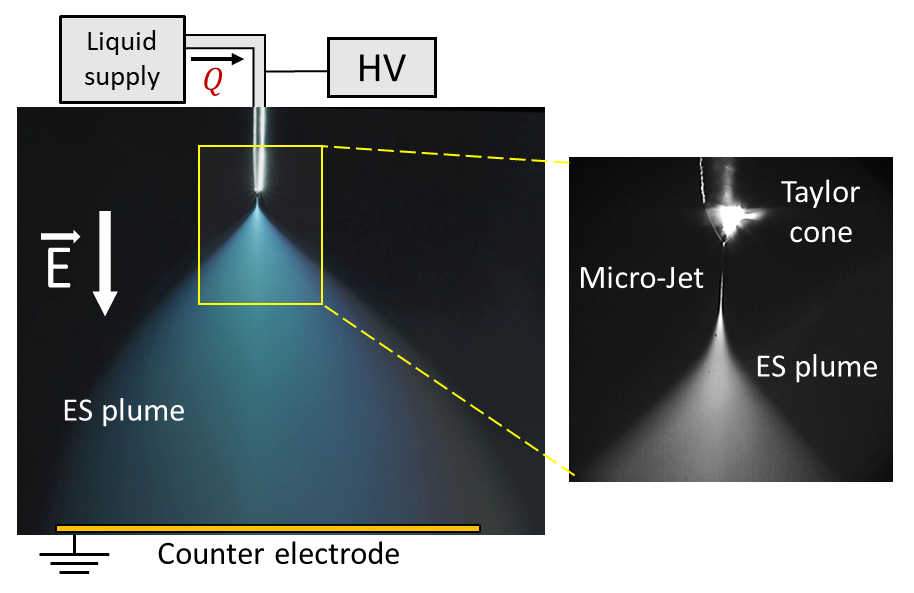
\includegraphics[width=.8\textwidth,trim=1 1 1 1,clip]{figures/Example.png}
    \caption{EXAMPLE OF FIGURE. Left: Conventional ES setup. Right: Droplet emission region.}
    \label{fig:ES_intro}
\end{figure}


% ==============================================
\subsection{Subsection}
\subsubsection{Subsubsection}

\blindtext % Remove this and write your text!


\subsubsection{Specific objectives}
\blindtext % Remove this and write your text!


% ==============================================
% \newpage
\section{First Approach: PID Controller}

\subsection{Time Response Analysis}

Before developing a proof-of-concept PID controller for the multinozzle, we first 
need to understad the time resonse of system to changes in the input.

\begin{figure}[h!]
    \centering
    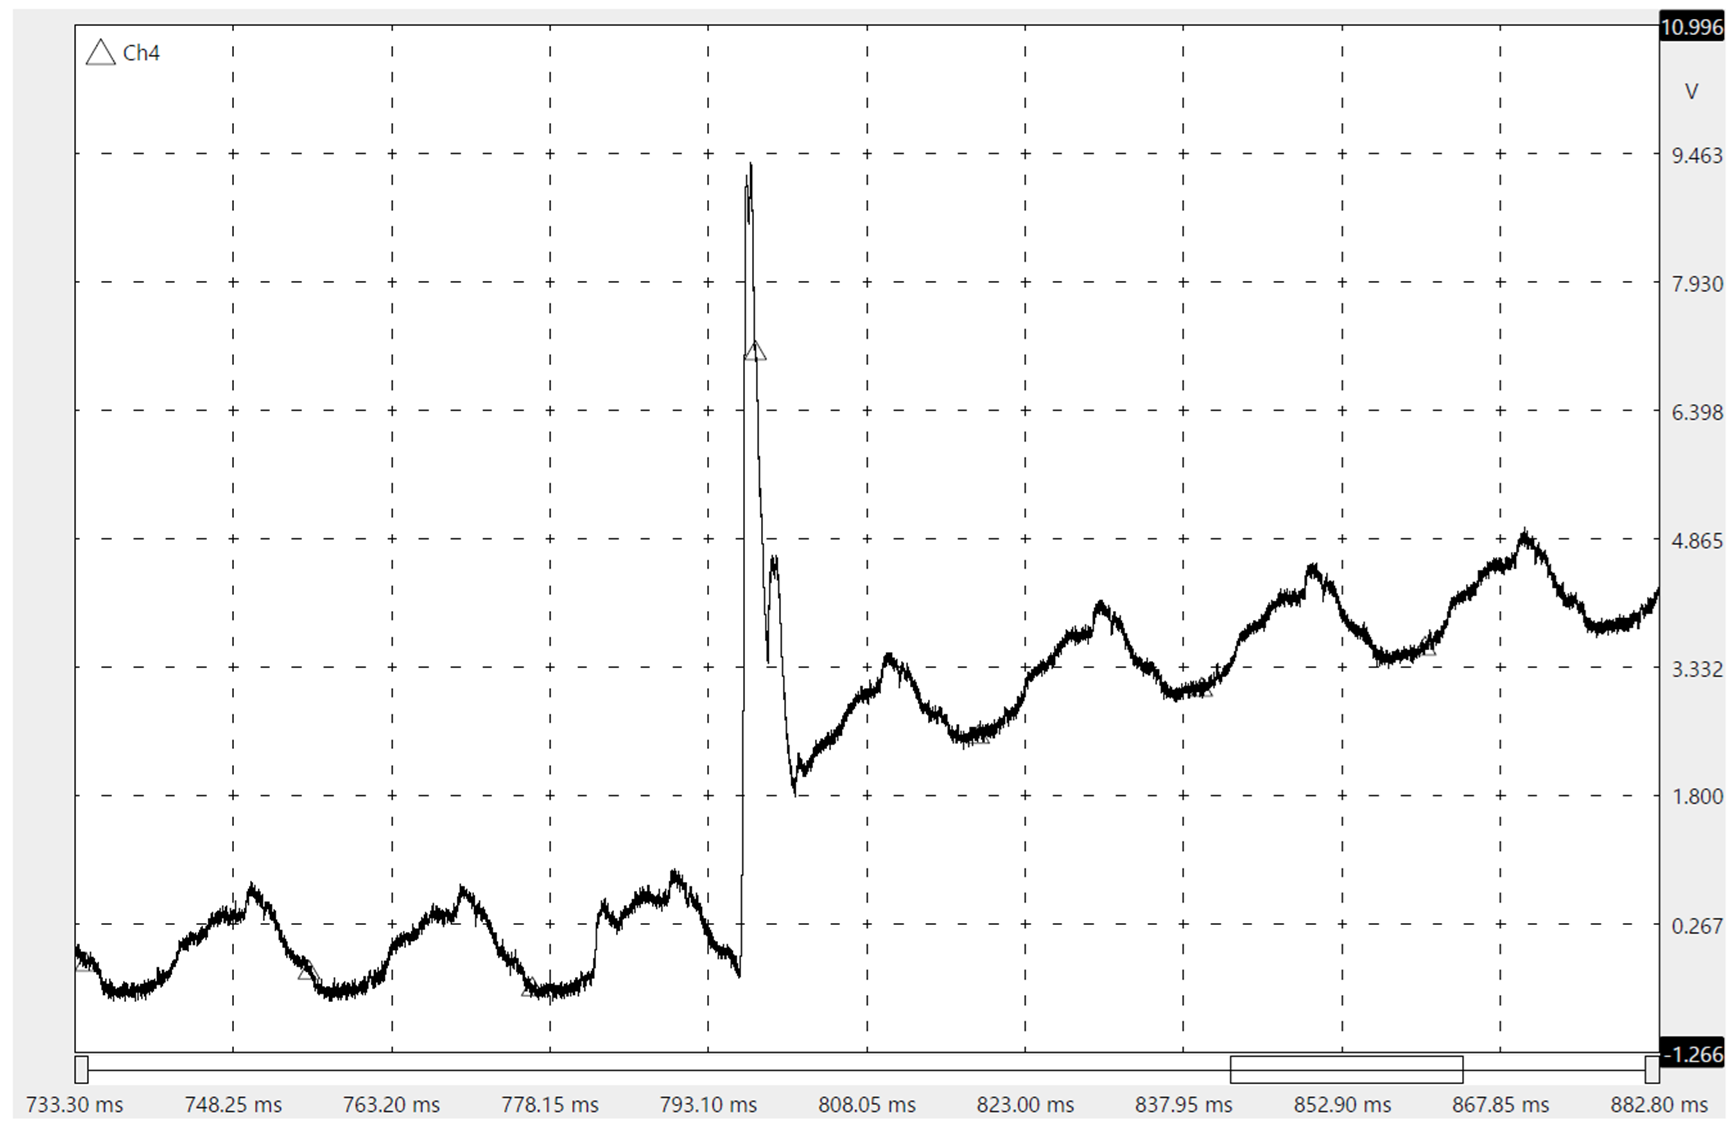
\includegraphics[width=.8\textwidth,trim=1 1 1 1,clip]{figures/inrush-current.png}
    \caption{Inrush current on the positive HV+ line.}
    \label{fig:inrush-current}
\end{figure}

\subsubsection{Subsubsection}

\blindtext % Remove this and write your text!

% ==============================================
% \newpage
\section{Second Approach: Current-based Classification and Control} 

Once identified the issues with the first approach, we attempted to design a 
controller based on the classification suggested by \hl{Verdoold (add reference)}.

The strategy adopted will be to first classify the electrospray mode by looking a current values 
on the system, and then experimentally design a controller that can move from an intermittent
to a cone-jet spray mode.

However, Verdoold's method was designed for the single nozzle, and it is not clear if we can 
extend his classification to a multinozzle configuration. Therefore, part of this work 
includes an attempt to extend his classification to the system developd by 
Gilbert.


\subsection{Measuring the currents by spray mode}

The first test done was to measure the current on all three lines of the sprayhead and 
verify if we see a pattern in the shape of current that can be used to classify the spray mode.
\autoref{fig:setup-three-currents-spray-mode} shows the setup used for this test.

\begin{figure}[h!]
    \centering
    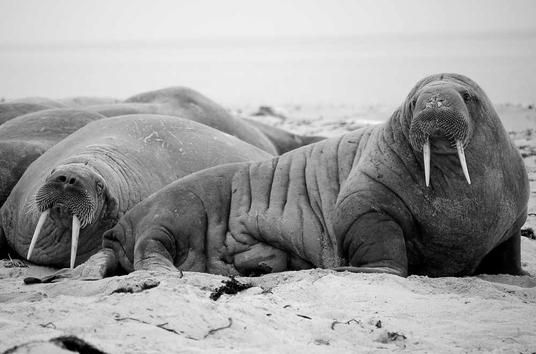
\includegraphics[width=.8\textwidth,trim=1 1 1 1,clip]{figures/lorem-picsum.jpg}
    \caption{Setup to measure all three currents on the sprayhead.}
    \label{fig:setup-three-currents-spray-mode}
\end{figure}

Using three oscilloscopes, all three currents were sampled at 5 kHz, collecting 20.000 samples of each
(totalling a 4 seconds time window). Notice that, although the oscilloscope has multiple channels, 
we cannot use the same oscilloscope as the channels are interconnected internally: the high voltage 
differences would damage the instrument. Therefore, we use one oscilloscope for each line. 

\autoref{fig:three-currents-spray-mode} shows the waveforms obtained for $\phi = 20 \un{mL/h}$.

\begin{figure}[h!]
    \centering
    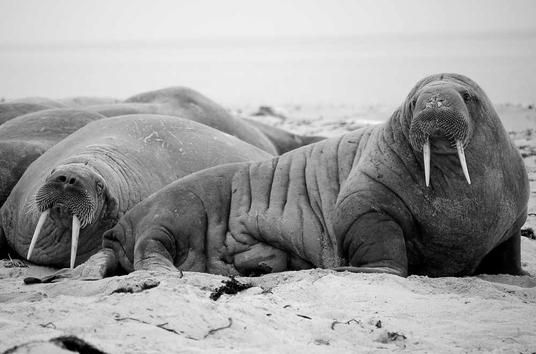
\includegraphics[width=.8\textwidth,trim=1 1 1 1,clip]{figures/lorem-picsum.jpg}
    \caption{$i_N$, $i_{GND}$ and $i_C$ by different spray modes.}
    \label{fig:three-currents-spray-mode}
\end{figure}

As we can see in \autoref{fig:three-currents-spray-mode}, we don't see a clear distinction in the shape of the current 
by different spray modes, in both time windows. We repeated the test for $\phi = 30 \un{mL/h}$ and $\phi = 50 \un{mL/h}$,
obtaining the same result, as shown in \autoref{fig:three-currents-spray-mode-all-flows}

\begin{figure}[h!]
    \centering
    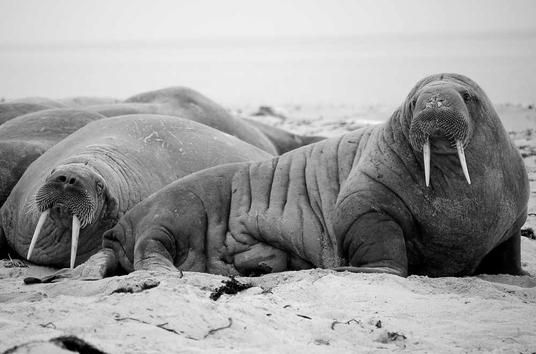
\includegraphics[width=.8\textwidth,trim=1 1 1 1,clip]{figures/lorem-picsum.jpg}
    \caption{$i_N$, $i_{GND}$ and $i_C$ by different spray modes for all $\phi$.}
    \label{fig:three-currents-spray-mode-all-flows}
\end{figure}

Without a clear distinction in the current waveforms it is not possible to continue with this approach.
Therefore, we need to first understand why we are not seing distinctions in the shape 
of the current, particularly between the intermittent and cone-jet spray modes, as it is clear in the 
literature that there should be a difference.

To do this, we'll begin by attempting to reproduce Verdoolds results, with the goal of isolating 
if the problem is our measurement strategy or if it is something related to the sprayhead itself.

\subsection{Reproducing Verdoold's Results}

\autoref{fig:verdoold-reproduce-setup} shows the setup used to reproduce Verdoolds approach.
We used a sampling frequency of 5 kHz and $\phi = 1 \un{mL/h}$. 

\begin{figure}[h!]
    \centering
    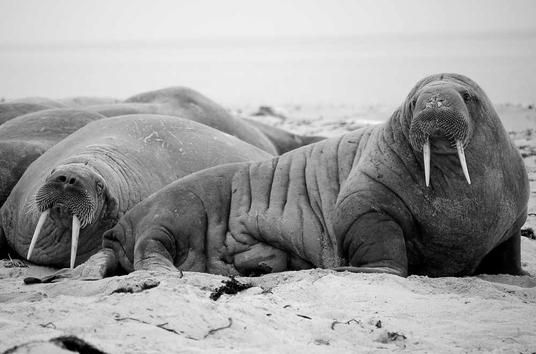
\includegraphics[width=.8\textwidth,trim=1 1 1 1,clip]{figures/lorem-picsum.jpg}
    \caption{Setup used to reproduce Verdoold's classification method.}
    \label{fig:verdoold-reproduce-setup}
\end{figure}

The results obtained are shown in \autoref{fig:verdoold-reproduce-results}. 

\begin{figure}[h!]
    \centering
    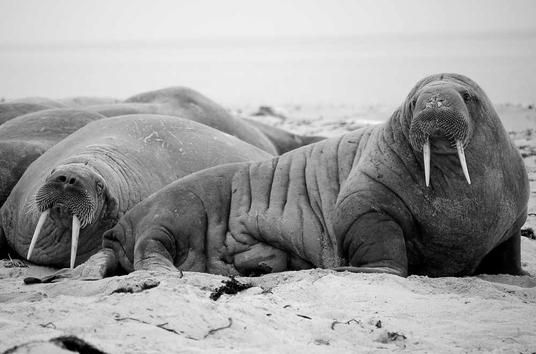
\includegraphics[width=.8\textwidth,trim=1 1 1 1,clip]{figures/lorem-picsum.jpg}
    \caption{Setup used to reproduce Verdoold's classification method.}
    \label{fig:verdoold-reproduce-results}
\end{figure}

As we can see in \autoref{fig:verdoold-reproduce-results}, we see a clear distinction between the spray modes, 
which is what we wish to see in the multinozzle. We can conclude that our measurement methodology can 
reproduce the results, therefore it must be something in the multinozzle that is "hiding" the intermittent spray 
signal.

Comparing the single nozzle setup on \autoref{fig:verdoold-reproduce-setup} and the multinozzle on \autoref{fig:setup-three-currents-spray-mode}, 
the most significant difference is indeed the presence of the crown. Therefore, let's begin by understand the influence 
of the crown on $i_{GND}$, which is the current that we know is capable of showing a distinction of spraying 
modes. 

\subsection{Crown influences on $i_{GND}$}

To understad the influence of the crown on the ground current, we'll use the same setup shown on 
\autoref{fig:setup-three-currents-spray-mode}, but we'll make $V_+ = 0 \un{V}$, $\phi = 0 \un{mL / h}$ and measure $i_{GND}$ for different
crown voltages. Since there is no flow 
and no positive voltage, we'll be measuring the current on the groung ring introduced by the crown only.

\autoref{fig:ignd-by-crown} shows the shape of $i_{GND}$ for different values of $V_-$.

\begin{figure}[h!]
    \centering
    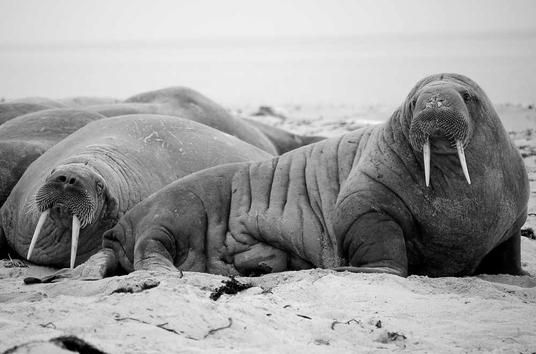
\includegraphics[width=.8\textwidth,trim=1 1 1 1,clip]{figures/lorem-picsum.jpg}
    \caption{$i_{GND}$ for different values of $V_-$. (a) Waveform and (b) standard deviation}
    \label{fig:ignd-by-crown}
\end{figure}

As seen of \autoref{fig:ignd-by-crown} (a), the crown alone introduces a signal on $i_{GND}$ starting
from $V_- = - 4 \un{kV}$, which increases in both average value and standard deviation as $V_-$ increases.
This is consistent with was happens at the crown: from $V_- = 4 \un{kV}$ the sharp needles 
of the crown begin to ionize the air, which produces that ions that can be 
directed to ground ring. This results in a current $i_{GND} > 0$ induced by the crown.

In addition, on \autoref{fig:ignd-by-crown} (b) we see that the standard deviation introduces by the crown
is significant. As we saw on \autoref{fig:verdoold-reproduce-results}, the intermittent spray mode 
presents peaks in the current signal in order of 100 nA, but the "noise" introduced by the 
crown alone is already over 50 nA. Therefore, it is reasonable to assuem that the reason we are
not seing a good distinction between the spray modes on \autoref{fig:three-currents-spray-mode} is 
because of this signal introduced by the crown.

\subsubsection{Atenuating Crown Influences on $i_{GND}$}

In order to verify the above hypothesis, we can try to reduce the influence of the crown
in the signal and verify if the intermittent signal becomes distinguishable. We can achieve this in two ways:

\begin{itemize}
    \item Reduce crown voltage
    \item Add filters in the signal
\end{itemize}

As we saw in \autoref{fig:ignd-by-crown} (a), the smaller $V_-$, the smaller the introduced 
noise in $i_{GND}$. Then, we can redo the measurements with a smaller crown voltage.

In addition, we can add digital filters in the oscilloscope to remove the following unwanted
frequencies:

\begin{itemize}
    \item 50 Hz frequency from the electric grid: use a stop band in the range 48 - 52 Hz
    \item All frequencies above 100 Hz: use low pass filter with cut-off frequency 100 Hz.
\end{itemize}

Note that, as shown by Verdoold, the intermittent peaks are usually under 100 Hz. Therefore, we can remove 
anything above this frequency from the signal as it is not what we wish to measure.

Using this, we get ...

\subsubsection{8 vs 16 Needle in the Crown}


\subsection{Optimizing Signal Acquisition}

In the previous sections, the signal was acquired using the minimum sampling frequency
suggested by the Verdoold of $f_s = 5 \un{kHz}$. A sample size of $N_s = 20.000$ was used to obtain a spectral resolution of 0.25 Hz
for frequency domain anaysis, also suggested by Verdoold as the minimum. However, talks with Gilbert showed that the sampling frequency was too
computationally expensive and the sample size was too slow, as it resulted in a sampling time window of 4 seconds, which is too large.

Therefore, to attempt to meet these requirements, we need to find the minimum sampling frequency and
minimum sample size that can still reliably distinguish the signal of the intermittent from the cone-jet.

To do this, we'll use the following method:

\begin{itemize}
    \item Collect a time window of 100 seconds for different values of $f_s$
    \item Break the 100 seconds into smaller time windows - denoted as $S_i$ - of size $S$. Note that $i = 1, 2, ...$
    \item Calculate the relevant statistical parameters in each $S_i$ and store these values
    \item Plot a boxplot of the calculated statistical parameters
\end{itemize}

We'll use the same setup shown in \hl{COMPLETE}. The resuls obtained are shown belon on ....

% ==============================================
% \newpage
\section{Conclusions} 

These are the conclusions:

\begin{itemize}
    \item \blindtext % Remove this and write your text!
    \item \blindtext % Remove this and write your text!
\end{itemize}


% ==============================================
\newpage    \pagestyle{plain}
\addcontentsline{toc}{chapter}{References} % 'References' will appear in the index.
\bibliography{references.bib}
% ==============================================
\end{document}